\chapter{Implementasi dan Pengujian}

\section{Implementasi}
Berdasarkan hasil analisis serta perancangan yang dituliskan pada Bab III, dilakukan implementasi ILE pada platform web KodeBareng. Dalam bab ini dijelaskan mengenai implementasi dan pengujian terhadap ILE yang dibuat.

\subsection{Batasan Implementasi}
Implementasi dilakukan menggunakan teknologi yang telah dipakai pada KodeBareng sebelumnya. Daftar teknologi dan \textit{framework} yang digunakan pada KodeBareng dapat dilihat pada \autoref{tab:tech-stack}.

\small
\begin{longtable}[c]{|>{\setlength{\baselineskip}{0.75\baselineskip}}p{0.3\linewidth}|>{\setlength{\baselineskip}{0.75\baselineskip}}p{0.4\linewidth}|}
  \caption{\textit{Tech stack} yang digunakan oleh KodeBareng} \label{tab:tech-stack}                               \\ \hline
  \rowcolor{gray!30}
  \textbf{Nama Sistem}                                     & \textbf{Teknologi / \textit{Framework} yang digunakan} \\ \hline
  \endfirsthead
  %
  \caption*{\autoref{tab:tech-stack} (lanjutan): \textit{Tech stack} yang digunakan oleh KodeBareng}                \\ \hline
  \rowcolor{gray!30}
  \textbf{Nama Sistem}                                     & \textbf{Teknologi / \textit{Framework} yang digunakan} \\ \hline
  \endhead
  %
  \textit{Frontend}                                        & NuxtJS, Cloudflare Pages                               \\ \hline
  \textit{Backend}                                         & ExpressJS, Linux, NodeJS, Docker                       \\ \hline
  CMS (\textit{Content Management System})                 & NextJS, Netlify                                        \\ \hline
  \textit{Autograder} (sekarang menjadi \textit{Executor}) & ExpressJS, Linux, NodeJS, Docker, Python 3.9           \\ \hline
\end{longtable}
\normalsize

Selain dari teknologi yang digunakan, terdapat juga batasan dari bahasa pemrograman yang dapat divisualisasikan eksekusinya yaitu Python sesuai dengan kelas pembelajaran pemrograman yang sudah ada pada platform web KodeBareng. Cakupan implementasi fitur bahasa pemrograman Python menggunakan rancangan dari bab sebelumnya pada \autoref{tab:ile-scope}.

\subsection{Eksplorasi PDB (\textit{Python Debugger})}

Sebelum dilakukan implementasi, dilakukan eksplorasi pada \textit{Python Debugger} (PDB) untuk mengetahui bagaimana implementasi ILE dapat berjalan khususnya pada pengolahan \textit{stack trace} dari PDB. Eksplorasi dilakukan untuk melihat perintah apa saja yang dapat dilakukan pada PDB, persiapan atau inisialisasi apa saja yang perlu dilakukan untuk mengolah data keluaran PDB, dan bagaimana cara mengambil data keluaran PDB yang diinginkan.

PDB memiliki serangkaian perintah yang dapat digunakan dalam melakukan \textit{debugging} seperti yang dapat dilihat pada \autoref{fig:pdb-commands}. Definisi dan kegunaan dari tiap perintah tersebut dapat dilihat pada dokumentasi PDB di \textcite{pdb2022documentation}. PDB dapat dijalankan dengan menggunakan perintah \verb|python -m pdb| atau \verb|python -m pdb -c "command"|.

\begin{figure}[H]
  \centering
  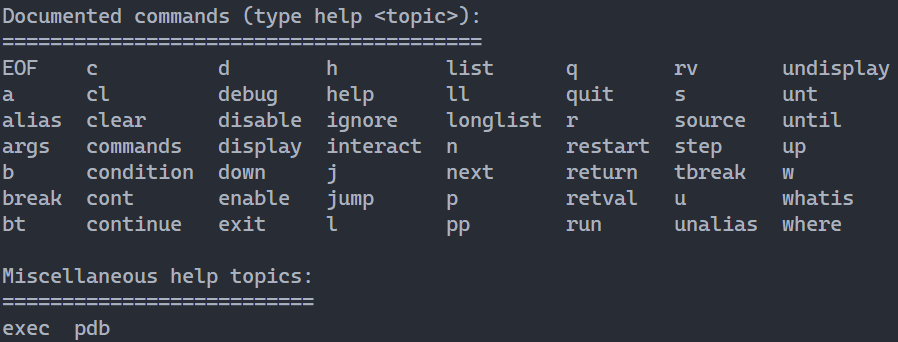
\includegraphics[width=0.7\textwidth]{chapter4/pdb-commands.png}
  \caption{Perintah-perintah yang dapat dieksekusi pada PDB} \label{fig:pdb-commands}
  Sumber: Penulis (2022)
\end{figure}

Dari sekian banyak perintah PDB yang dapat dipakai, terdapat beberapa perintah yang digunakan pada komponen Executor untuk mendapatkan data \textit{stack trace} yang diinginkan. Perintah-perintah tersebut beserta contoh keluarannya dapat dilihat pada \autoref{tab:pdb-commands-primitive}. Hasil dari eksekusi perintah itu kemudian diolah oleh komponen Parser untuk diekstrak data-data pentingnya saja serta untuk penentuan logika pengecekan komponen Parser.

\footnotesize
\begin{longtable}[c]{|l|l|>{\raggedright\arraybackslash\setlength{\baselineskip}{0.75\baselineskip}}p{0.3\linewidth}|>{\raggedright\arraybackslash\setlength{\baselineskip}{0.75\baselineskip}}p{0.45\linewidth}|}
  \caption{Perintah primitif PDB yang dipakai oleh komponen Executor} \label{tab:pdb-commands-primitive}                                                                                                                                                                                                                                                                                                                                                                                                                                                                                                                                                                                                                                                                                                                                                                                                                                                                                                                                                                                                                                                                                                                                                             \\ \hline
  \rowcolor[HTML]{C0C0C0}
  \multicolumn{1}{|c|}{\cellcolor[HTML]{C0C0C0}\textbf{Perintah}} & \multicolumn{1}{>{\centering\arraybackslash\setlength{\baselineskip}{0.75\baselineskip}}p{0.1\linewidth}|}{\cellcolor[HTML]{C0C0C0}\textbf{Nama perintah}} & \multicolumn{1}{c|}{\cellcolor[HTML]{C0C0C0}\textbf{Deskripsi}}                                                                                               & \multicolumn{1}{c|}{\cellcolor[HTML]{C0C0C0}\textbf{Contoh output}}                                                                                                                                                                                                                                                                                                                                                                                                                                                                                                                                                                                                                                                                                                                                                                                                 \\ \hline
  \endfirsthead
  %
  \caption*{\autoref{tab:pdb-commands-primitive} (lanjutan): Perintah primitif PDB yang dipakai oleh komponen Executor} \label{tab:pdb-commands-primitive}                                                                                                                                                                                                                                                                                                                                                                                                                                                                                                                                                                                                                                                                                                                                                                                                                                                                                                                                                                                                                                                                                                           \\ \hline
  \rowcolor[HTML]{C0C0C0}
  \multicolumn{1}{|c|}{\cellcolor[HTML]{C0C0C0}\textbf{Perintah}} & \multicolumn{1}{>{\centering\arraybackslash\setlength{\baselineskip}{0.75\baselineskip}}p{0.1\linewidth}|}{\cellcolor[HTML]{C0C0C0}\textbf{Nama perintah}} & \multicolumn{1}{c|}{\cellcolor[HTML]{C0C0C0}\textbf{Deskripsi}}                                                                                               & \multicolumn{1}{c|}{\cellcolor[HTML]{C0C0C0}\textbf{Contoh output}}                                                                                                                                                                                                                                                                                                                                                                                                                                                                                                                                                                                                                                                                                                                                                                                                 \\ \hline
  \endhead
  %
  \verb|s|                                                        & Next/Step                                                                                                                                                  & Melanjutkan langkah eksekusi program dan mengeluarkan permintaan input, keluaran dari program, atau informasi baris yang sedang dieksekusi.                   & \begin{tabular}[t]{@{}>{\raggedright\arraybackslash\setlength{\baselineskip}{0.75\baselineskip}\scriptsize}p{\linewidth}@{}@{}m{0pt}@{}}{[}&\\[-1ex]   '\textbf{the result is}',&\\[-1ex]   '{[}35, 300{]}',  '\textgreater /1\_simpleCalculation.py(22)\textless{}module\textgreater{}()',&\\[-1ex]   '-\textgreater print(wrapper)',&\\[-1ex]   '(Pdb) '&\\[-1ex] {]}\end{tabular}                                                                                                                                                                                                                                                                                                                                                                                                                                        \\ \hline
  \verb|c|                                                        & Continue                                                                                                                                                   & Melanjutkan langkah eksekusi program hingga program selesai, debugger menemukan breakpoint, atau terdapat error pada program.                                 & \begin{tabular}[t]{@{}>{\raggedright\arraybackslash\setlength{\baselineskip}{0.75\baselineskip}\scriptsize}p{\linewidth}@{}@{}m{0pt}@{}}{[}&\\[-1ex]   'Traceback (most recent call last):',&\\[-1ex]   '  File "/python3.8/pdb.py", line 1705, in main',&\\[-1ex]   '    pdb.\_runscript(mainpyfile)',&\\[-1ex]   '  File "/python3.8/pdb.py", line 1573, in \_runscript',&\\[-1ex]   '    self.run(statement)',&\\[-1ex]   '  File "/python3.8/bdb.py", line 580, in run',&\\[-1ex]   '    exec(cmd, globals, locals)',&\\[-1ex]   '  File "\textless{}string\textgreater{}", line 1, in \textless{}module\textgreater{}',&\\[-1ex]   '  File "/error.py", line 6, in \textless{}module\textgreater{}',&\\[-1ex]   '    print(123) / 0',&\\[-1ex]   "TypeError: unsupported operand type(s) for /: 'NoneType' and 'int'",&\\[-1ex]   ''&\\[-1ex] {]}\end{tabular} \\ \hline
  \verb|w|                                                        & Where                                                                                                                                                      & Memperlihatkan stack frame apa saja yang terdapat pada program, baris keberapa dari program yang sedang dieksekusi, dan return value dari fungsi apabila ada. & \begin{tabular}[t]{@{}>{\raggedright\arraybackslash\setlength{\baselineskip}{0.75\baselineskip}\scriptsize}p{\linewidth}@{}@{}m{0pt}@{}}{[}&\\[-1ex]   '  /python3.8/bdb.py(580)run()',&\\[-1ex]   '-\textgreater exec(cmd, globals, locals)',&\\[-1ex]   '  \textless{}string\textgreater{}(1)\textless{}module\textgreater{}()',&\\[-1ex]   \textbf{'  /12\_listSum.py(10)\textless{}module\textgreater{}()'},&\\[-1ex]   \textbf{'-\textgreater total = listSum(myList)'},&\\[-1ex]   \textbf{'\textgreater /12\_listSum.py(5)listSum()'},&\\[-1ex]   \textbf{'-\textgreater (f, rest) = numbers'},&\\[-1ex]   '(Pdb) '&\\[-1ex] {]}\end{tabular}                                                                                                                                                                                               \\ \hline
  \verb|return|                                                   & Return                                                                                                                                                     & Mengeluarkan eksekusi kode program dari suatu fungsi yang sedang dijalankan atau mengecek apakah program telah selesai                                        & \begin{tabular}[t]{@{}>{\raggedright\arraybackslash\setlength{\baselineskip}{0.75\baselineskip}\scriptsize}p{\linewidth}@{}@{}m{0pt}@{}}{[}&\\[-1ex]   '\textbf{The program finished and will be restarted}',  '\textgreater /12\_listSum.py(1)\textless{}module\textgreater{}()',&\\[-1ex]   '-\textgreater def listSum(numbers):',&\\[-1ex]   '(Pdb) '&\\[-1ex] {]}\end{tabular}                                                                                                                                                                                                                                                                                                                                                                                                                                                                                  \\ \hline
  \verb|q|                                                        & Quit                                                                                                                                                       & Mematikan program                                                                                                                                             & -                                                                                                                                                                                                                                                                                                                                                                                                                                                                                                                                                                                                                                                                                                                                                                                                                                                                   \\ \hline
  \verb|p|                                                        & Print                                                                                                                                                      & menampilkan isi dari suatu variabel                                                                                                                           & \begin{tabular}[t]{@{}>{\raggedright\arraybackslash\setlength{\baselineskip}{0.75\baselineskip}\scriptsize}p{\linewidth}@{}@{}m{0pt}@{}}\textbf{Command: p \_\_EXECUTOR}&\\[-1ex] {[}&\\[-1ex]   "\textbf{\{'locals': \textless{}built-in function locals\textgreater{}, 'globals': \textless{}built-in function globals\textgreater{}\}}",&\\[-1ex]   '(Pdb) '&\\[-1ex] {]}\end{tabular}                                                                                                                                                                                                                                                                                                                                                                                                                                     \\ \hline
\end{longtable}
\normalsize

Selain dari perintah-perintah tersebut, terdapat rangkaian perintah yang digunakan oleh komponen Executor yang telah didefinisikan sebelumnya pada tahap inisialisasi komponen Executor. Perintah-perintah tersebut digunakan agar data yang didapatkan oleh PDB semakin rinci dan dapat diolah dengan mudah karena telah diubah menjadi bentuk JSON. Daftar perintah, kegunaan, beserta contoh keluarannya dapat dilihat pada \autoref{tab:pdb-commands-functions}.

\footnotesize
\begin{longtable}[c]{|>{\raggedright\arraybackslash\setlength{\baselineskip}{0.75\baselineskip}\scriptsize}p{0.15\linewidth}|>{\raggedright\arraybackslash\setlength{\baselineskip}{0.75\baselineskip}}p{0.1\linewidth}|>{\raggedright\arraybackslash\setlength{\baselineskip}{0.75\baselineskip}}p{0.3\linewidth}|>{\raggedright\arraybackslash\setlength{\baselineskip}{0.75\baselineskip}}p{0.45\linewidth}|}
  \caption{Perintah olahan untuk PDB yang dipakai oleh komponen Executor} \label{tab:pdb-commands-functions}                                                                                                                                                                                                                                                                                                                                                                                                                                                                                                                                                                                                                                                                                                                                                                                                                           \\ \hline
  \rowcolor[HTML]{C0C0C0}
  \multicolumn{1}{|c|}{\cellcolor[HTML]{C0C0C0}\textbf{Perintah}}                & \multicolumn{1}{>{\raggedright\arraybackslash\setlength{\baselineskip}{0.75\baselineskip}}p{0.1\linewidth}|}{\cellcolor[HTML]{C0C0C0}\textbf{Nama perintah}} & \multicolumn{1}{c|}{\cellcolor[HTML]{C0C0C0}\textbf{Deskripsi}}                                                                                                                    & \multicolumn{1}{c|}{\cellcolor[HTML]{C0C0C0}\textbf{Contoh output}}                                                                                                                                                                                                                                                                                                                                                                                                                             \\ \hline
  \endfirsthead
  %
  \caption*{\autoref{tab:pdb-commands-functions} (lanjutan): Perintah olahan untuk PDB yang dipakai oleh komponen Executor}                                                                                                                                                                                                                                                                                                                                                                                                                                                                                                                                                                                                                                                                                                                                                                                                            \\ \hline
  \rowcolor[HTML]{C0C0C0}
  \multicolumn{1}{|c|}{\cellcolor[HTML]{C0C0C0}\textbf{Perintah}}                & \multicolumn{1}{>{\raggedright\arraybackslash\setlength{\baselineskip}{0.75\baselineskip}}p{0.1\linewidth}|}{\cellcolor[HTML]{C0C0C0}\textbf{Nama perintah}} & \multicolumn{1}{c|}{\cellcolor[HTML]{C0C0C0}\textbf{Deskripsi}}                                                                                                                    & \multicolumn{1}{c|}{\cellcolor[HTML]{C0C0C0}\textbf{Contoh output}}                                                                                                                                                                                                                                                                                                                                                                                                                             \\ \hline
  \endhead
  %
  \begin{spverbatim}!'__exception__' in __EXECUTOR ['globals']()\end{spverbatim} & Check Error                                                                                                                                                  & Mengecek apakah terdapat error saat melanjutkan langkah eksekusi kode. Menghasilkan keluaran \verb|True| atau \verb|False| serta mengeluarkan output berupa error yang ditemukan.  & \begin{tabular}[t]{@{}>{\raggedright\arraybackslash\setlength{\baselineskip}{0.75\baselineskip}\scriptsize}p{\linewidth}@{}@{}m{0pt}@{}}{[}&\\[-1ex]   \textbf{"TypeError: unsupported operand type(s) for /: 'NoneType' and 'int'"},&\\[-1ex]   '\textgreater /error.py(6)\textless{}module\textgreater{}()',&\\[-1ex]   '-\textgreater print(123) / 0',&\\[-1ex]   \textbf{'True'},  '(Pdb) '&\\[-1ex] {]}\end{tabular}                                                                       \\ \hline
  \begin{spverbatim}extractType(x)\end{spverbatim}                               & Extract Type                                                                                                                                                 & Mendapatkan tipe dari variabel yang dimasukkan ke dalam parameternya. Menghasilkan keluaran JSON.                                                                                  & \begin{tabular}[t]{@{}>{\raggedright\arraybackslash\setlength{\baselineskip}{0.75\baselineskip}\scriptsize}p{\linewidth}@{}@{}m{0pt}@{}}\{&\\[-1ex]   "type": "int"&\\[-1ex] \}\end{tabular}                                                                                                                                                                                                                                                                                                    \\ \hline
  \begin{spverbatim}deepGetInfo (data)\end{spverbatim}                           & Deep Get Info                                                                                                                                                & Mendapatkan nilai, tipe, dan id dari suatu variabel dan memakai rekursi untuk mendapatkan informasi tersebut dari tipe data berjenis Collection. Menghasilkan keluaran JSON.       & \begin{tabular}[t]{@{}>{\raggedright\arraybackslash\setlength{\baselineskip}{0.75\baselineskip}\scriptsize}p{\linewidth}@{}@{}m{0pt}@{}}\{&\\[-1ex]   "z": \{&\\[-1ex]     "value": {[}&\\[-1ex]       \{ "value": 35, "id": 9790048, "type": "int" \},&\\[-1ex]       \{ "value": 300, "id": 140165068398096, "type": "int" \}&\\[-1ex]     {]},&\\[-1ex]     "id": 140165068695616,&\\[-1ex]     "type": "list"&\\[-1ex]   \}&\\[-1ex] \}\end{tabular}                                        \\ \hline
  \begin{spverbatim}generateGet Fields( fieldType, type)\end{spverbatim}         & Get Fields                                                                                                                                                   & Menghasilkan kode eksekusi untuk mendapatkan data variabel yang diperlukan menggunakan deepGetInfo dan extractType dari locals() dan globals() Python. Menghasilkan keluaran JSON. & \begin{tabular}[t]{@{}>{\raggedright\arraybackslash\setlength{\baselineskip}{0.75\baselineskip}\scriptsize}p{\linewidth}@{}@{}m{0pt}@{}}{[}&\\[-1ex]   `'\{"tripX": \{"value": 1953125.0, "id": 140634468547152, "type": "float"\}\}'`,&\\[-1ex]   `'\{"swap": \{"value": "\_\_FUNCTION\_\_", "id": 140634467574544, "type": "function"\}\}'`,&\\[-1ex]   `'\{"math": \{"value": "\_\_MODULE\_\_", "id": 140634467665616, "type": "module"\}\}'`,&\\[-1ex]   '(Pdb) '&\\[-1ex] {]}\end{tabular} \\ \hline
\end{longtable}
\normalsize

Hasil eksplorasi PDB akan digunakan pada komponen Executor dan komponen Parser yang akan dijelaskan pada bagian berikut (\autoref{ssec:implementasi-sistem-eksekutor}) menggunakan alur rancangan yang telah dibuat di bab sebelumnya pada \autoref{fig:activity-executor}.

\subsection{Implementasi Sistem Eksekutor} \label{ssec:implementasi-sistem-eksekutor}
Sistem Eksekutor menggunakan \textit{tech stack} berupa ExpressJS dengan Typescript yang dijalankan pada NodeJS menggunakan kakas \textit{nodemon}. Sistem tersebut kemudian diisolasi menggunakan Docker dengan \textit{image} Debian 10 dan dilakukan instalasi Python 3.9. Terdapat juga kakas berupa \textit{swagger} yang digunakan untuk dokumentasi rute-rute yang terdapat pada sistem ini.

\subsubsection{Modifikasi Komponen Controller}
Pada sistem ini sudah terdapat \textit{controller} pada tiap bagian rute untuk mengolah data yang diberikan. Pada Tugas Akhir ini, ditambahkan rute untuk melakukan visualisasi serta \textit{controller} untuk mengolah data tersebut. \textit{Controller} mendapatkan masukan berupa kode program berupa \textit{string} serta input berupa \verb|array of string| untuk diberikan pada program yang dieksekusi. Kemudian, \textit{Controller} melakukan pengecekan apakah kode diperbolehkan untuk dieksekusi, lalu menuliskan kode pada file Python sementara. Setelah itu, \textit{controller} menjalankan \textit{helper} berupa Komponen Executor dan Parser dengan memberikan masukan berupa lokasi \textit{file} kode program serta \textit{input} yang akan diberikan pada program.

% [\hl{TODO: MASUKIN CONTOH HASIL INPUT CONTROLLER UNTUK KOMPONEN EXECUTOR DAN PARSER}]
\subsubsection{Implementasi Komponen Executor}
Komponen Executor merupakan komponen yang digunakan untuk mengeksekusi kode program menggunakan PDB. Komponen ini membutuhkan masukan berupa lokasi \textit{file} berisi kode program yang akan dieksekusi serta \textit{input} yang akan diberikan kepada program. Terdapat 3 tahapan utama dalam komponen ini, yaitu tahap inisialisasi, tahap pengecekan, serta tahap pengumpulan data.

Tahap inisialisasi adalah tahap menginjeksi kode tambahan ke dalam eksekusi Python untuk keperluan Komponen Executor dan Parser. Pada tahap ini, dimasukkan kode untuk mengubah keluaran Python menjadi JSON agar dapat diolah oleh NodeJS. Selain itu, terdapat juga fungsi-fungsi tambahan untuk mendapatkan tipe data pada Python serta melakukan \textit{deep iteration} untuk mendapatkan informasi tipe data serta id dari variabel yang bertipe \textit{sequence} atau \textit{hashmap}. Tahap inisialisasi hanya dilakukan sekali untuk setiap kode program yang dijalankan.

Setelah inisialisasi dijalankan, dilakukan tahap pengecekan yaitu untuk mengecek apakah eksekusi program sedang berada di luar kode program yang seharusnya karena terkadang PDB menjalankan kode program pada modul \textit{standard library} (\textit{built-in module}). Apabila program sedang mengeksekusi baris diluar kode program (penentuan dilakukan oleh Komponen Parser), maka Komponen Executor akan mengeksekusi perintah untuk kembali keluar modul tersebut dan kembali pada kode program awal. Setelah itu, Komponen Executor akan melanjutkan langkah eksekusi tanpa melalui tahapan pengumpulan data.

Apabila program lolos dari tahap pengecekan (program tidak berada di luar kode program), maka dilakukan tahap pengumpulan data. Tahap pengumpulan data adalah tahap pengumpulan \textit{fields} yang berada pada \textit{runtime memory} seperti variabel, fungsi dan metode, serta modul yang telah dimuat. Tahap ini terbagi menjadi 3 subtahap, yaitu tahap \verb|Local|, \verb|Global|, dan \verb|Stack|. Subtahap \verb|Lokal| adalah subtahap mengeksekusi perintah untuk mengumpulkan \textit{fields} pada memori lokal suatu \textit{stack frame}. Subtahap \verb|Global| adalah subtahap mengeksekusi perintah untuk mengumpulkan \textit{fields} pada memori global suatu program. Subtahap \verb|Stack| adalah subtahap mengeksekusi perintah untuk mengumpulkan data pada \textit{stack frame} berupa baris kode yang sedang dieksekusi, \textit{return value}, serta daftar \textit{frame} yang tersimpan pada \textit{stack frame}.Hasil keluaran dari seluruh perintah tersebut akan diolah oleh Komponen Parser.

Setelah Komponen Executor dan Parser melewati tahap pengumpulan data dan tidak terjadi error, maka Komponen Executor akan melanjutkan langkah eksekusi kode sekaligus perintah yang digunakan untuk pengecekan \textit{error}, serta me-\textit{reset} data-data dan tahapan-tahapan yang dilakukan lalu kembali pada tahap pengecekan. Apabila terdapat error selama tahap pengumpulan data, maka Komponen Executor akan mematikan program yang sedang dieksekusi. Apabila jumlah langkah atau lama waktu eksekusi sudah melebihi batas yang telah ditentukan, maka Komponen Executor juga akan mematikan program yang sedang dieksekusi.

% [\hl{TODO: MASUKIN CONTOH HASIL KELUARAN KOMPONEN EXECUTOR }]

\subsubsection{Implementasi Komponen Parser}
Komponen Parser merupakan komponen yang digunakan untuk mengolah hasil keluaran Komponen Executor. Komponen ini juga menentukan logika dan langkah yang akan diambil oleh Komponen Executor. Komponen ini membutuhkan masukan berupa \verb|array of string| yang merupakan hasil keluaran Komponen Executor yang telah dipisahkan tiap barisnya. Terdapat 2 tahapan utama dalam komponen ini, yaitu tahap pengecekan dan tahap pengumpulan data.

Tahap pengecekan dilakukan bersamaan dengan Komponen Executor melakukan tahap pengecekan. Pada tahap ini, terdapat beberapa subtahap yaitu pengecekan \textit{input}, pengecekan \textit{output}, serta pengecekan eksekusi \textit{built-in module}.

Pada subtahap pengecekan \textit{input}, dilakukan pengecekan terhadap \textit{signature output} dari PDB serta pengecekan waktu eksekusi suatu baris. Apabila tidak ditemukan \textit{signature output} dari PDB atau waktu eksekusi suatu baris melebihi batas, maka komponen ini akan memasukkan \textit{input} (melalui Komponen Executor) sesuai dengan \textit{input} yang dberikan oleh \textit{controller}. Apabila tidak ada \textit{input} yang diberikan oleh \textit{controller} atau \textit{input} yang diberikan oleh \textit{controller} kurang dari jumlah input yang dibutuhkan, maka Komponen Parser akan memasukkan \textit{event} untuk meminta tambahan input dan mematikan program yang dieksekusi.

Setelah itu, dilakukan subtahap pengecekan \textit{output} untuk mengecek dan mengolah apabila program mengeluarkan \textit{output} atau \textit{error} setelah melanjutkan langkah eksekusi. Apabila program mengeluarkan \textit{error}, maka Komponen Parser akan mengolah \textit{error} dan \textit{traceback} yang dikeluarkan dan menyimpannya ke dalam \textit{event} lalu mematikan program. Apabila program mengeluarkan \textit{output}, maka Komponen Parser akan mengolah \textit{output} tersebut dan memasukkannya ke dalam daftar \textit{output} program.

Kemudian, dilakukan subtahap pengecekan eksekusi \textit{built-in module} yang telah dijelaskan pada Komponen Executor sebelumnya. Komponen Parser akan mengecek hasil keluaran dari perintah yang dimasukkan oleh Komponen Executor, kemudian apabila terdeteksi \textit{error} maka Komponen Parser tidak akan mengolah data hingga Komponen Executor melanjutkan langkah eksekusi program.

Setelah seluruh tahapan dalam tahap pengecekan selesai, Komponen Parser akan memasuki tahap pengumpulan data yang tahapannya sama dengan tahapan pengumpulan data yang terdapat pada Komponen Executor. Hasil keluaran Komponen Executor diolah dengan mengolah keluaran JSON. Apabila keluaran tersebut tidak dapat diolah sebagai JSON, maka Komponen Parser akan menghasilkan \textit{error}, disimpan sebagai \textit{event} lalu mematikan program. Setelah semua subtahap pengumpulan data dilakukan, Komponen Parser akan mengolah seluruh hasil pengumpulan data ke dalam daftar \verb|ExecutionResult| yang akan dikembalikan kepada \textit{controller} saat program telah selesai atau dimatikan dan menjadi hasil yang dapat divisualisasikan pada Sistem Frontend.

% [\hl{TODO: MASUKKAN CONTOH HASIL KELUARAN KOMPONEN PARSER}]

\subsection{Implementasi Backend}
\subsubsection{Implementasi Komponen Helper}
Komponen Helper merupakan komponen yang digunakan untuk mendeteksi perintah-perintah yang tidak diperbolehkan eksekusi pada kode. Apabila tidak terdapat perintah yang dilarang pada kode, maka kode diteruskan kepada sistem Executor dan mengembalikan hasilnya. Apabila terdapat perintah yang dilarang pada kode, maka kode akan ditolak dan tidak akan dieksekusi.


\subsection{Implementasi Frontend}

\subsubsection{Implementasi Komponen Web IDE}
Komponen Web IDE dibuat menggunakan Monaco Editor yang dibuat oleh Microsoft. Komponen ini dapat memperlihatkan \textit{syntax highlighting} pada kode, menunjukkan angka baris, serta navigasi menggunakan \textit{scrollbar} yang memiliki \textit{overview} dari seluruh kode program.

Komponen ini terhubung pada Komponen Visualizer untuk menampilkan dekorator-dekorator saat visualisasi eksekusi kode berlangsung. Tampilan hasil implementasi Web IDE dapat dilihat pada \autoref{fig:web-ide}.

\begin{figure}[H]
  \centering
  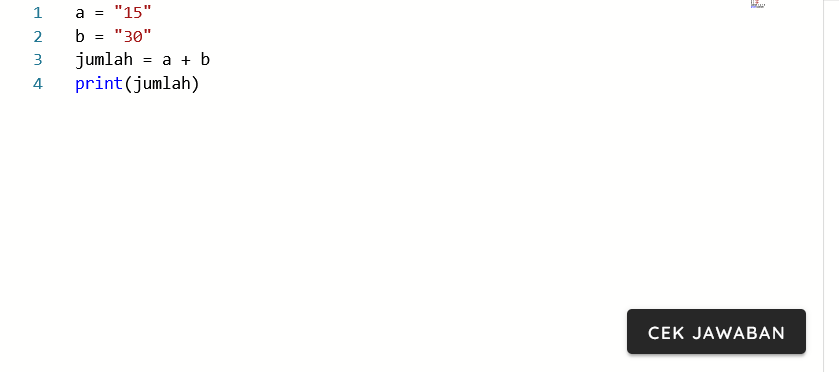
\includegraphics[width=0.7\textwidth]{chapter4/web-ide.png}
  \caption{Tampilan Antarmuka Web IDE} \label{fig:web-ide}
  Sumber: Penulis (2022)
\end{figure}

\subsubsection{Implementasi Komponen Visualizer}
Komponen Visualizer merupakan komponen yang dapat memvisualisasikan hasil olahan \textit{stack trace} suatu kode. Komponen ini dapat berinteraksi dengan Web IDE untuk menunjukkan lokasi eksekusi suatu langkah dengan memberikan warna pada baris eksekusi, serta membuat tabel data pada memori pada setiap \textit{stack frame}. Pengguna dapat mengubah alur maju mundur visualisasi, melihat isi data pada setiap \textit{stack frame}, serta melihat perubahan pada data dalam memori.

Komponen ini dapat dimasukkan pada bagian materi pembelajaran dan bagian persoalan seperti Kuis dan Latihan Kode. Komponen ini dapat dinon-aktifkan apabila tidak diperbolehkan untuk digunakan. Tampilan hasil implementasi Visualizer dapat dilihat pada \autoref{fig:ile-materi} dan \autoref{fig:ile-soal}.

\begin{figure}[H]
  \centering
  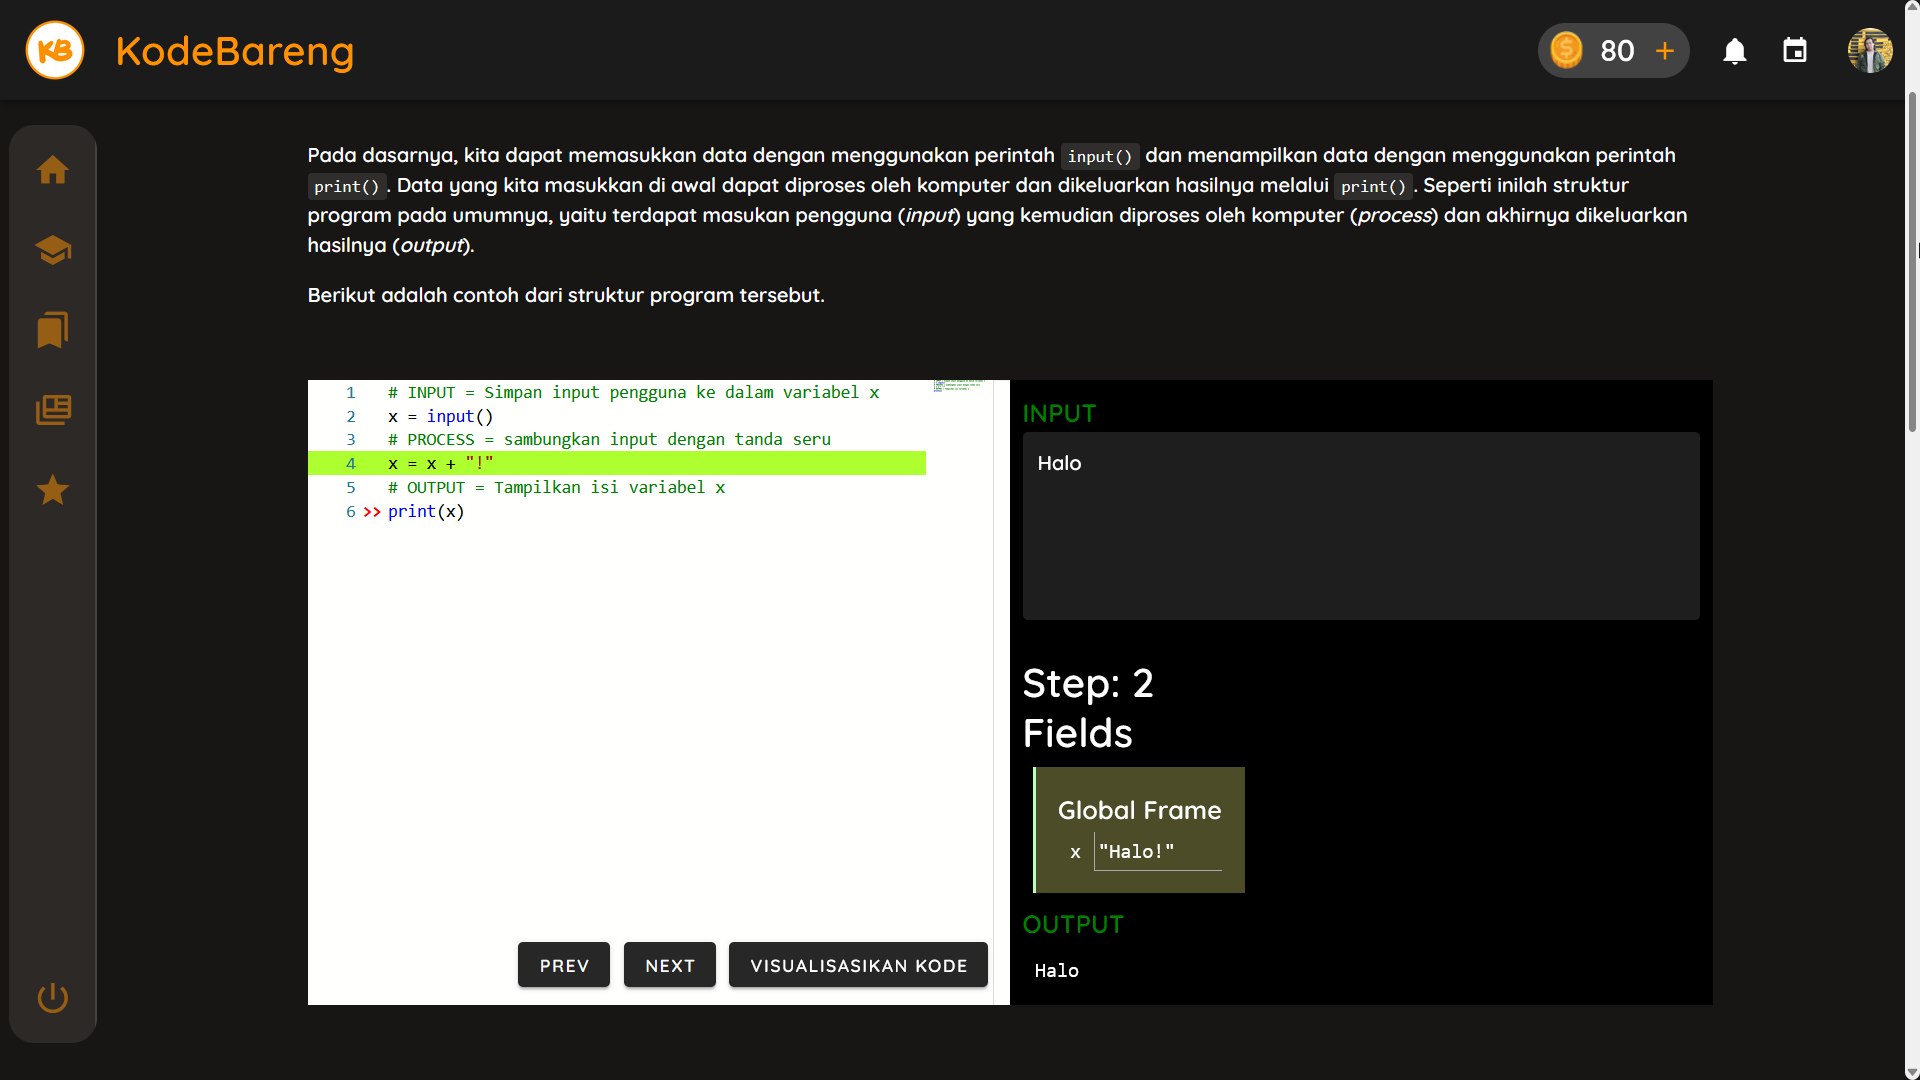
\includegraphics[width=0.7\textwidth]{chapter4/ile-materi.png}
  \caption{Tampilan antarmuka Visualizer pada materi pembelajaran} \label{fig:ile-materi}
  Sumber: Penulis (2022)
\end{figure}
\begin{figure}[H]
  \centering
  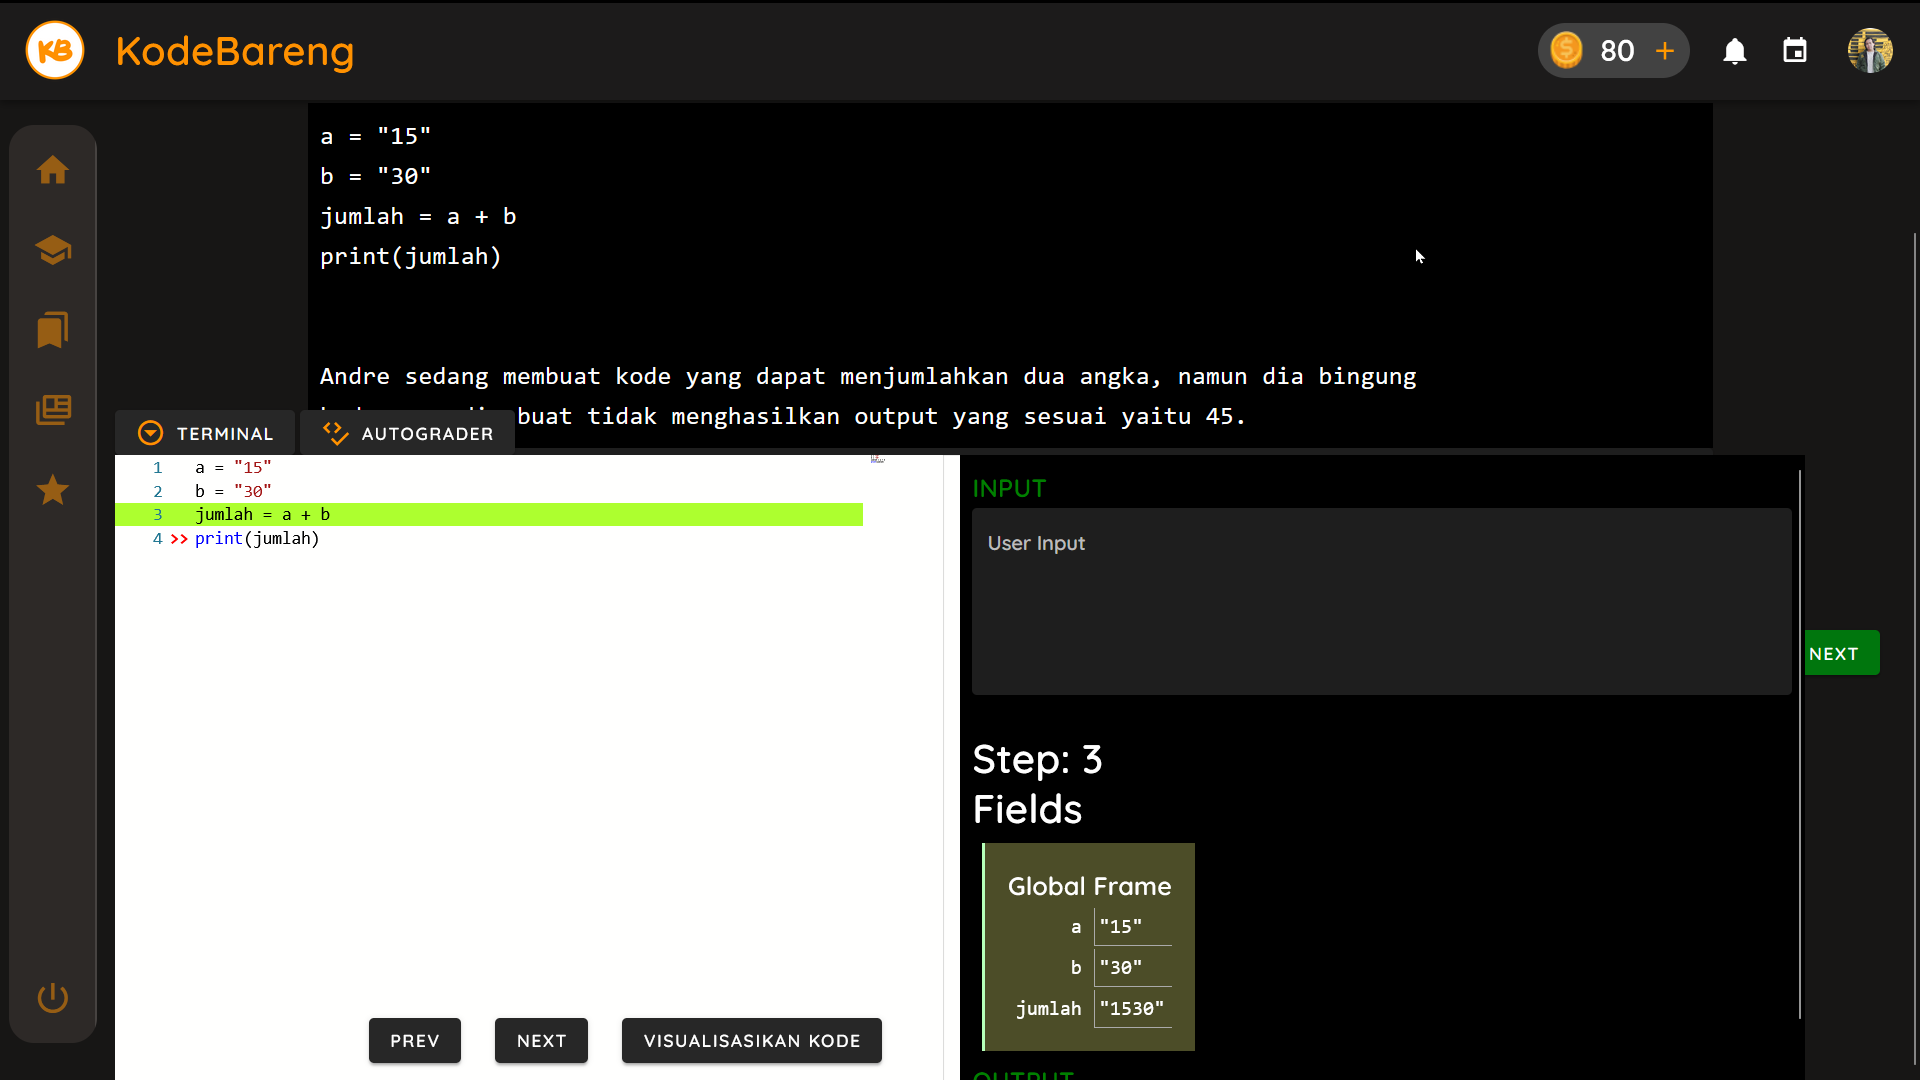
\includegraphics[width=0.7\textwidth]{chapter4/ile-soal.png}
  \caption{Tampilan antarmuka Visualizer pada persoalan Latihan Kode} \label{fig:ile-soal}
  Sumber: Penulis (2022)
\end{figure}

\section{Pengujian}

\subsection{Tujuan Pengujian}
Tujuan dari pengujian ini adalah untuk memastikan bahwa ILE yang diimplementasikan telah sesuai dengan spesifikasi kebutuhan yang telah dibuat sebelumnya serta mendapatkan data terkait dampak ILE yang telah dibuat terhadap pemahaman pelajar mengenai konsep serta alur kerja eksekusi kode program.

\subsection{Lingkungan Pengujian}
Lingkungan pengujian terbagi menjadi 2 yaitu lingkungan komputer dan lingkungan eksperimen pengguna (\textit{user experiment}). Lingkungan komputer digunakan untuk menjalankan fungsional sistem, sementara lingkungan eksperimen pengguna digunakan untuk melakukan eksperimen pengguna pada komputer peserta eksperimen masing-masing.

Pengujian spesifikasi fungsional sistem dilakukan pada komputer server KodeBareng dengan spesifikasi pada \autoref{tab:lingkungan-server} untuk menjalankan Sistem Backend dan Sistem Executor.

\small
\begin{longtable}[c]{|l|l|}
  \caption{Lingkungan pengujian komputer server} \label{tab:lingkungan-server}                \\ \hline
  \rowcolor{gray!30}
  \textbf{Komponen} & \textbf{Keterangan}                                                     \\ \hline
  \endfirsthead
  %
  \caption*{\autoref{tab:lingkungan-server} (lanjutan): Lingkungan pengujian komputer server} \\ \hline
  \rowcolor{gray!30}
  \textbf{Komponen} & \textbf{Keterangan}                                                     \\ \hline
  \endhead
  %
  Prosesor          & Intel(R) Xeon(R) CPU E5-2660 0 @ 2.20GHz                                \\ \hline
  Memori            & 2GB                                                                     \\ \hline
  Storage           & 32GB                                                                    \\ \hline
  Sistem Operasi    & Ubuntu 20.04.4 LTS                                                      \\ \hline
\end{longtable}
\normalsize

Eksperiment pengguna dilakukan pada komputer peserta eksperimen masing-masing secara daring dengan pengarahan menggunakan platform \textit{Google Meet}.

\subsection{Skenario dan Hasil Pengujian}

\subsubsection{Pengujian Fungsional}
Pengujian fungsional dilakukan berdasarkan spesifikasi kebutuhan fungsional dan non-fungsional ILE pada \autoref{tab:srs-fungsional} dan \autoref{tab:srs-nonfungsional} pada \autoref{sec:analisis-kebutuhan}. Skenario dan hasil pengujian dapat dilihat pada \autoref{tab:pengujian-fungsional} dan \autoref{tab:pengujian-nonfungsional} berikut.

\small
\begin{longtable}[c]{|l|>{\setlength{\baselineskip}{0.75\baselineskip}}p{0.5\linewidth}|>{\setlength{\baselineskip}{0.75\baselineskip}}p{0.2\linewidth}|}
  \caption{Skenario dan hasil pengujian fungsional} \label{tab:pengujian-fungsional}                                     \\ \hline
  \rowcolor{gray!30}
  \textbf{ID} & \textbf{Skenario}                                                                       & \textbf{Hasil} \\ \hline
  \endfirsthead
  %
  \caption*{\autoref{tab:pengujian-fungsional} (lanjutan): Skenario dan hasil pengujian fungsional}                      \\ \hline
  \rowcolor{gray!30}
  \textbf{ID} & \textbf{Skenario}                                                                       & \textbf{Hasil} \\ \hline
  \endhead
  %
  KB-F-01     & Pelajar memasukkan kode program pada sistem                                             & Diterima       \\ \hline
  KB-F-02     & Pelajar memasukkan input program pada sistem                                            & Diterima       \\ \hline
  KB-F-03     & Pelajar dapat menjalankan kode                                                          & Diterima       \\ \hline
  KB-F-04     & Pelajar dapat melihat hasil visualisasi eksekusi kode                                   & Diterima       \\ \hline
  KB-F-05     & Pelajar mendapat penilaian dari hasil eksekusi kode                                     & Diterima       \\ \hline
  KB-F-06     & Pelajar mendapat \textit{hint} kesalahan pada kode program                              & Diterima       \\ \hline
  KB-F-07     & Pelajar dapat melihat pesan error pada program                                          & Diterima       \\ \hline
  KB-F-08     & Sistem menolak kode pelajar apabila terdapat perintah-perintah yang tidak diperbolehkan & Diterima       \\ \hline
  KB-F-09     & Sistem menilai kode program menggunakan \textit{test case}                              & Diterima       \\ \hline
  KB-F-10     & Sistem mengolah \textit{stack trace} eksekusi program                                   & Diterima       \\ \hline
  KB-F-11     & Administrator menentukan perintah-perintah yang tidak diperbolehkan                     & Diterima       \\ \hline
  KB-F-12     & Administrator memasukkan konten materi pembelajaran                                     & Diterima       \\ \hline
  KB-F-13     & Administrator membuat soal pemrograman                                                  & Diterima       \\ \hline
  KB-F-14     & Administrator memasukkan \textit{test case} soal pemrograman                            & Diterima       \\ \hline
  KB-F-15     & Administrator memasukkan \textit{hint} kesalahan yang dapat ditampilkan pada soal       & Diterima       \\ \hline
\end{longtable}
\normalsize

\small
\begin{longtable}[c]{|l|>{\setlength{\baselineskip}{0.75\baselineskip}}p{0.6\linewidth}|l|}
  \caption{Skenario dan hasil pengujian non-fungsional} \label{tab:pengujian-nonfungsional}                \\ \hline
  \rowcolor{gray!30}
  \textbf{ID} & \textbf{Skenario}                                         & \textbf{Hasil}                 \\ \hline
  \endfirsthead
  %
  \caption*{\autoref{tab:pengujian-nonfungsional} (lanjutan): Skenario dan hasil pengujian non-fungsional} \\ \hline
  \rowcolor{gray!30}
  \textbf{ID} & \textbf{Skenario}                                         & \textbf{Hasil}                 \\ \hline
  \endhead
  %
  KB-NF-01    & Sistem mengembalikan hasil eksekusi paling lama 10 detik. & Diterima                       \\ \hline
  KB-NF-02    & Sistem dapat diuji menggunakan beragam kode program       & Diterima                       \\ \hline
  KB-NF-03    & Sistem menolak kode berbahaya                             & Diterima                       \\ \hline
\end{longtable}
\normalsize

\subsubsection{Eksperimen Pengguna (\textit{User Experiment})}

Eksperimen pengguna dilakukan terhadap faktor pemahaman pelajar mengenai konsep pemrograman serta alur kerja eksekusi kode program. Maka dari itu, pengujian dilakukan berdasarkan pengujian pada \textcite{mayer1981psychology} untuk perlakuan pemberian model konkret kepada pelajar saat pembelajaran berlangsung serta \textcite{moons2013pilot} untuk cara pengukuran pemahaman konsep. Sebagai batasan, eksperimen ini hanya akan dilakukan pada orang yang baru belajar pemrograman atau belum pernah belajar pemrograman sebelumnya.

Pengujian ini dilakukan pada platform web KodeBareng dengan menggunakan kelas pembelajaran khusus untuk melakukan pengujian. Pengujian dilakukan pada 2 grup dengan masing-masing grup memiliki minimal 10 peserta eksperimen, yaitu grup kontrol dan grup perlakuan. Grup kontrol mendapatkan materi pembelajaran tanpa adanya integrasi ILE visualisasi eksekusi kode, sementara grup perlakuan mendapatkan materi pembelajaran yang terdapat integrasi ILE visualisasi eksekusi kode. Setiap grup mendapatkan materi pembelajaran yang sama serta kuesioner setelah melakukan pembelajaran.

Materi yang diberikan terbagi menjadi 3 modul yaitu modul Pengenalan Python Dasar, Variabel dan Tipe Data, serta Operator dan Ekspresi. Pada masing-masing modul, terdapat 2 tahapan yaitu tahap pembelajaran dan tahap persoalan. Pada tahap pembelajaran, materi diberikan melalui teks, gambar dan ILE (khusus pada grup perlakuan, pada grup kontrol hanya diperlihatkan teks kode serta \textit{input/output}-nya). Pada tahap persoalan, terdapat 2 jenis persoalan yaitu kuis dan latihan kode. Soal kuis adalah soal sederhana bertipe pilihan ganda, sementara soal latihan kode adalah soal yang memberikan bagian suatu kode program yang harus diubah oleh peserta untuk memenuhi objektif yang diberikan. Soal kuis dinilai secara benar atau salah (1/0) dan soal latihan kode akan dinilai menggunakan SOLO Level dengan kategori penilaian seperti pada \autoref{tab:solo-level} namun hanya mencapai level ke-4 karena pembelajaran tidak sampai diujikan pada domain lainnya. SOLO (Structure of Observed Learning Outcomes) adalah salah satu jenis taksonomi dalam pendidikan yang mengukur tingkat abstraksi pemahaman konsep yang telah dicapai oleh peserta didik \parencite{moons2013pilot}. Pada setiap akhir modul, terdapat 2 soal kuis dan 1 soal latihan kode. Setiap tahapan harus diselesaikan terlebih dahulu sebelum peserta dapat melanjutkan pembelajaran.

Pada kuesioner, terdapat 2 pertanyaan menggunakan \textit{likert scale} yaitu "Apakah visualisasi kode membuatmu lebih memahami kode yang dijalankan?" dan "Apakah visualisasi kode membantumu menjawab kuis dan latihan soal?", serta 1 pertanyaan bertipe isian paragraf yaitu "Pendapat atau saran untuk fitur visualisasi eksekusi kode". Selain pertanyaan yang berkaitan dengan ILE, terdapat juga pertanyaan umum lainnya seperti pengalaman pembelajaran di KodeBareng dan pendapat saran untuk pembelajaran di KodeBareng. Kuesioner digunakan sebagai data kualitatif tambahan untuk mengukur dampak dari ILE dari sisi penggunanya. Pertanyaan kuesioner terkait ILE hanya dijawab oleh peserta grup perlakuan.

Selain dari materi pembelajaran dan kuesioner, terdapat juga data tambahan berupa \textit{event} yang disimpan selama eksperimen berlangsung untuk mengukur waktu pembelajaran pada suatu tahap, berapa banyak interaksi yang dilakukan pelajar pada ILE, serta jawaban-jawaban yang di-\textit{submit} oleh pelajar saat menjawab persoalan Kuis dan Latihan Kode.

\subsection{Prosedur Eksperimen Pengguna}
Sebelum pengujian, disebarkan formulir pendaftaran eksperimen yang dilakukan pada Sabtu, 28 Mei 2022. Selain data kontak dan demografis, data mengenai pengalaman pembelajaran pemrograman sebelumnya juga diambil. Pengujian dilakukan dalam rentan waktu 4 hari, yaitu dimulai pada 29 Mei hingga 1 Juni 2022. Orang yang telah mendaftar eksperimen kemudian dikontak untuk dilakukan penjadwalan eksperimen. Dari 42 orang yang mendaftar eksperimen melalui formulir tersebut, terdapat 25 orang yang merespon dan dapat menjadwalkan eksperimen sehingga menjadi peserta eksperimen yang sah (data terlampir pada \autoref{appendix:data-pendaftaran}). Demografis peserta eksperimen dapat dilihat pada \autoref{fig:demografis-usia}, \autoref{fig:demografis-pendidikan}, serta \autoref{fig:demografis-kelamin}. Kemudian, peserta dipetakan menjadi 13 orang grup perlakuan dan 12 orang grup kontrol.

\begin{figure}[H]
  \centering
  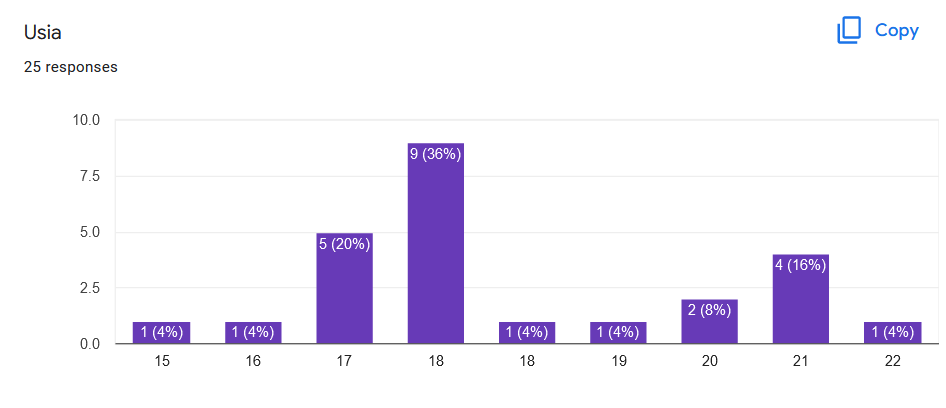
\includegraphics[width=0.7\textwidth]{chapter4/demografis-usia.png}
  \caption{Demografis usia peserta eksperimen} \label{fig:demografis-usia}
  Sumber: Penulis (2022)
\end{figure}
\begin{figure}[H]
  \centering
  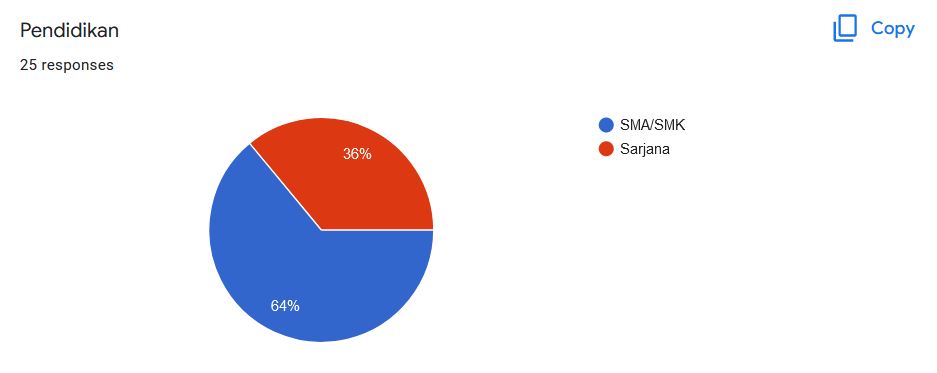
\includegraphics[width=0.7\textwidth]{chapter4/demografis-pendidikan.png}
  \caption{Demografis tahap pendidikan peserta eksperimen} \label{fig:demografis-pendidikan}
  Sumber: Penulis (2022)
\end{figure}
\begin{figure}[H]
  \centering
  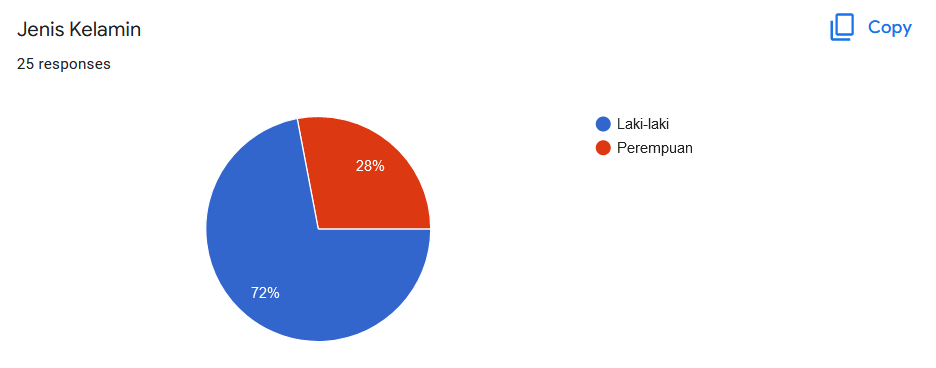
\includegraphics[width=0.7\textwidth]{chapter4/demografis-kelamin.png}
  \caption{Demografis jenis kelamin peserta eksperimen} \label{fig:demografis-kelamin}
  Sumber: Penulis (2022)
\end{figure}

Eksperimen dilakukan secara daring menggunakan platform \textit{Google Meet}. Peserta dibagikan tautan \textit{Google Meet} sesuai dengan jadwal kloter eksperimen yang sudah ditentukan sebelumnya. Peserta diminta menggunakan laptop/komputer saat melakukan eksperimen. Setelah seluruh peserta dalam satu kloter telah masuk ke dalam \textit{Google Meet}, peserta dibagikan tautan menuju formulir kuesioner untuk mengisi identitas diri terlebih dahulu. Kemudian, peserta diarahkan menuju situs KodeBareng, membuat akun KodeBareng menggunakan akun Google, lalu membuka kelas sesuai dengan grup masing-masing. Sebelum memulai pembelajaran, peserta diberikan arahan mengenai cara belajar di KodeBareng serta instruksi untuk melakukan pembelajaran sesuai dengan kecepatan masing-masing selama 1 jam. Khusus untuk peserta pada grup perlakuan, mereka diberikan pengenalan cara menggunakan ILE yang telah disediakan selama pembelajaran. Setelah 1 jam berlalu, selesai tidak selesai peserta akan diminta untuk menghentikan pembelajaran lalu melanjutkan mengisi kuesioner.

\section{Analisis Hasil Pengujian} \label{sec:analisis-hasil-pengujian}

\subsection{Analisis Data Kuesioner}
Karena pertanyaan kuesioner hanya diberikan kepada peserta yang telah memakai ILE, terdapat 13 peserta yang memberikan respon terhadap pertanyaan kuesioner. Terdapat 2 pertanyaan kuesioner yang diberikan, yaitu pertanyaan untuk mengukur dampak ILE terhadap pemahaman kode yang dijalankan serta pertanyaan untuk mengukur dampak ILE terhadap penyelesaian soal kuis dan latihan kode.

Berikut \autoref{fig:kuesioner-memahami} dan \autoref{tab:kuesioner1-statistik} adalah grafik serta tabel perhitungan statistik dari pertanyaan kuesioner pertama yang dirangkum dari data pada \autoref{appendix:data-kuesioner-kontrol} untuk grup kontrol dan \autoref{appendix:data-kuesioner-perlakuan} untuk grup perlakuan.

\begin{figure}[H]
  \centering
  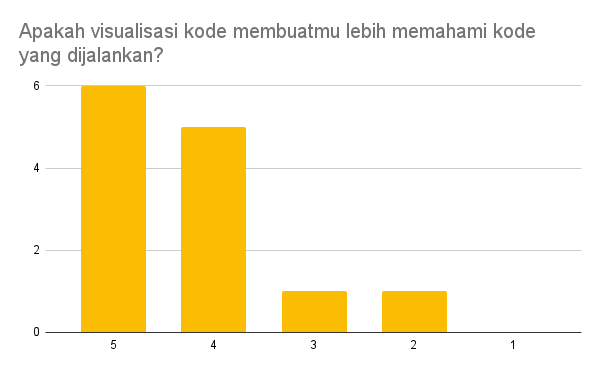
\includegraphics[width=0.7\textwidth]{chapter4/kuesioner-memahami.png}
  \caption{Apakah ILE membantu memahami kode?} \label{fig:kuesioner-memahami}
  Sumber: Penulis (2022)
\end{figure}

\small
\begin{longtable}[c]{|l|>{\setlength{\baselineskip}{0.75\baselineskip}}p{0.5\linewidth}|}
  \caption{Hasil perhitungan statistik deskriptif pada respon kuesioner pertanyaan pertama} \label{tab:kuesioner1-statistik}                                                 \\ \hline
                           & Apakah visualisasi kode membuatmu lebih memahami kode yang dijalankan?                                                                          \\ \hline
  \endfirsthead
  %
  \caption*{\autoref{tab:kuesioner1-statistik} (lanjutan): Hasil perhitungan statistik deskriptif pada respon kuesioner pertanyaan pertama} \label{tab:kuesioner1-statistik} \\ \hline
                           & Apakah visualisasi kode membuatmu lebih memahami kode yang dijalankan?                                                                          \\ \hline
  \endhead
  %
  Mean                     & 4.230769                                                                                                                                        \\ \hline
  Standard Error           & 0.25705                                                                                                                                         \\ \hline
  Median                   & 4                                                                                                                                               \\ \hline
  Mode                     & 5                                                                                                                                               \\ \hline
  Standard Deviation       & 0.926809                                                                                                                                        \\ \hline
  Sample Variance          & 0.858974                                                                                                                                        \\ \hline
  Kurtosis                 & 1.524332                                                                                                                                        \\ \hline
  Skewness                 & -1.27368                                                                                                                                        \\ \hline
  Range                    & 3                                                                                                                                               \\ \hline
  Minimum                  & 2                                                                                                                                               \\ \hline
  Maximum                  & 5                                                                                                                                               \\ \hline
  Sum                      & 55                                                                                                                                              \\ \hline
  Count                    & 13                                                                                                                                              \\ \hline
  Confidence Level(95,0\%) & 0.560065                                                                                                                                        \\ \hline
\end{longtable}
\normalsize

Berdasarkan \autoref{fig:kuesioner-memahami} dan \autoref{tab:kuesioner1-statistik}, dapat disimpulkan bahwa mayoritas peserta eksperimen pada grup perlakuan merasa ILE membantu mereka dalam memahami kode yang dijalankan. \textit{Confidence Interval} dengan \textit{Confidence Level} 95\% jatuh pada kisaran nilai 3.671-4.791.

Berikut \autoref{fig:kuesioner-soal} dan \autoref{tab:kuesioner2-statistik} adalah grafik serta tabel perhitungan statistik dari pertanyaan kuesioner kedua.

\begin{figure}[H]
  \centering
  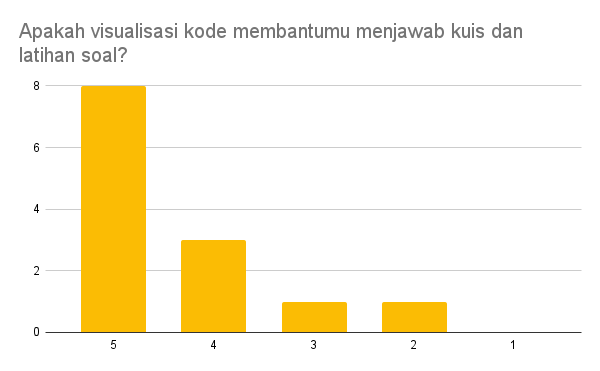
\includegraphics[width=0.7\textwidth]{chapter4/kuesioner-soal.png}
  \caption{Apakah ILE membantu menjawab latihan soal?} \label{fig:kuesioner-soal}
  Sumber: Penulis (2022)
\end{figure}

\small
\begin{longtable}[c]{|l|>{\setlength{\baselineskip}{0.75\baselineskip}}p{0.5\linewidth}|}
  \caption{Hasil perhitungan statistik deskriptif pada respon kuesioner pertanyaan kedua} \label{tab:kuesioner2-statistik}                                                 \\ \hline
                           & Apakah visualisasi kode membantumu menjawab kuis dan latihan soal?                                                                            \\ \hline
  \endfirsthead
  %
  \caption*{\autoref{tab:kuesioner2-statistik} (lanjutan): Hasil perhitungan statistik deskriptif pada respon kuesioner pertanyaan kedua} \label{tab:kuesioner2-statistik} \\ \hline
                           & Apakah visualisasi kode membantumu menjawab kuis dan latihan soal?                                                                            \\ \hline
  \endhead
  %
  Mean                     & 4.384615                                                                                                                                      \\ \hline
  Standard Error           & 0.266469                                                                                                                                      \\ \hline
  Median                   & 5                                                                                                                                             \\ \hline
  Mode                     & 5                                                                                                                                             \\ \hline
  Standard Deviation       & 0.960769                                                                                                                                      \\ \hline
  Sample Variance          & 0.923077                                                                                                                                      \\ \hline
  Kurtosis                 & 2.096086                                                                                                                                      \\ \hline
  Skewness                 & -1.6125                                                                                                                                       \\ \hline
  Range                    & 3                                                                                                                                             \\ \hline
  Minimum                  & 2                                                                                                                                             \\ \hline
  Maximum                  & 5                                                                                                                                             \\ \hline
  Sum                      & 57                                                                                                                                            \\ \hline
  Count                    & 13                                                                                                                                            \\ \hline
  Confidence Level(95,0\%) & 0.580587                                                                                                                                      \\ \hline
\end{longtable}
\normalsize

Berdasarkan \autoref{fig:kuesioner-soal} dan \autoref{tab:kuesioner2-statistik}, dapat disimpulkan bahwa mayoritas peserta eksperimen pada grup perlakuan merasa ILE membantu mereka dalam menjawab kuis serta latihan soal yang diberikan. \textit{Confidence Interval} dengan \textit{Confidence Level} 95\% jatuh pada kisaran nilai 3.804-4.965.

Pada \autoref{fig:kuesioner-average} berikut ditampilkan perbandingan rata-rata respon kuesioner pertanyaan pertama dan kedua.

\begin{figure}[H]
  \centering
  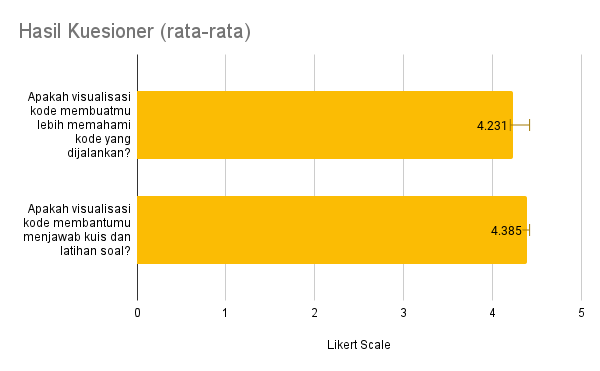
\includegraphics[width=0.9\textwidth]{chapter4/kuesioner-average.png}
  \caption{Perbandingan rata-rata hasil kuesioner ILE} \label{fig:kuesioner-average}
  Sumber: Penulis (2022)
\end{figure}

Apabila dibandingkan dengan pertanyaan kuesioner pertama, ILE memberikan dampak lebih tinggi dalam membantu memecahkan persoalan. Namun, apabila dilihat dari saran-saran serta pendapat yang diberikan, ILE banyak digunakan untuk memahami proses alur kerja suatu kode. Beberapa peserta pada grup kontrol bahkan memberikan saran untuk memasukkan fitur eksekusi kode pada materi pembelajaran, yang sebenarnya sudah diterapkan pada grup perlakuan. Meskipun dengan jumlah respon yang sedikit, hal ini menjadi indikasi bahwa ILE memiliki dampak dalam pembelajaran pemrograman bagi pemula.

\subsection{Analisis Data Eksperimen}
Setelah dilakukan eksperimen terhadap 25 peserta, didapatkan data penyelesaian modul tiap peserta yang dilampirkan pada \autoref{appendix:data-modul1-jawaban} untuk modul 1 dan \autoref{appendix:data-modul2-jawaban} untuk modul 2. Namun, pada hari pertama eksperimen terdapat kesalahan teknis dalam pengambilan data sehingga data beberapa peserta tidak tersimpan. Terdapat 3 peserta pada grup perlakuan yang datanya hilang akibat kesalahan pada basis data, sehingga peserta eksperimen yang dapat diolah datanya berkurang menjadi 22 peserta dengan pembagian 10 peserta grup perlakuan dan 12 peserta grup kontrol.

Dari 22 peserta eksperimen, seluruh peserta berhasil menyelesaikan modul pertama (Pengenalan Python Dasar). Namun pada modul kedua (Tipe Data), terdapat 4 peserta (3 peserta grup perlakuan dan 1 peserta grup kontrol) yang tidak berhasil menyelesaikan modul tersebut (tidak berhasil mencapai tahap persoalan) karena keterbatasan waktu eksperimen, sehingga peserta eksperimen yang berhasil menyelesaikan modul kedua berjumlah 18 orang dengan pembagian 7 peserta grup perlakuan dan 11 peserta grup kontrol. Kemudian, peserta yang dapat menyelesaikan modul ketiga (Operator dan Ekspresi) berjumlah 13 orang dengan pembagian 3 peserta grup perlakuan dan 10 peserta grup kontrol. 1 peserta grup kontrol dan 1 peserta grup perlakuan tidak berhasil mencapai tahap persoalan, 2 peserta grup perlakuan hanya mencapai soal kuis kedua (tidak menyelesaikan soal kuis ketiga dan soal latihan kode), dan 1 peserta grup perlakuan hanya mencapai soal kuis ketiga (tidak menyelesaikan soal latihan kode). Karena kurangnya data jumlah peserta eksperimen pada modul 3 serta terdapat perbedaan jumlah peserta grup perlakuan dan grup kontrol yang cukup besar, maka modul yang akan dipakai datanya hanya modul 1 dan modul 2. Data mengenai jumlah peserta yang menyelesaikan tiap modulnya dapat dilihat pada \autoref{tab:user-experiment-completion}.

\small
\begin{longtable}[c]{|l|ll|ll|}
  \caption{Pemetaan penyelesaian modul peserta eksperimen} \label{tab:user-experiment-completion}                                                                                                                                                                                                                                                                                                                                                                                                                                    \\ \hline
  \rowcolor[HTML]{C0C0C0}
  \multicolumn{1}{|c|}{\cellcolor[HTML]{C0C0C0}}                                 & \multicolumn{2}{c|}{\cellcolor[HTML]{C0C0C0}\textbf{\begin{tabular}[c]{@{}c@{}}Total peserta yang\\ menyelesaikan modul\end{tabular}}} & \multicolumn{2}{c|}{\cellcolor[HTML]{C0C0C0}\textbf{\begin{tabular}[c]{@{}c@{}}Total peserta pemula{\color{red}*} yang\\menyelesaikan modul\end{tabular}}}                                                                                                                                   \\ \cline{2-5}
  \rowcolor[HTML]{C0C0C0}
  \multicolumn{1}{|c|}{\multirow{-2}{*}{\cellcolor[HTML]{C0C0C0}\textbf{Modul}}} & \multicolumn{1}{c|}{\cellcolor[HTML]{C0C0C0}\textbf{Control}}                                                                          & \multicolumn{1}{c|}{\cellcolor[HTML]{C0C0C0}\textbf{Treatment}}                                                                                                        & \multicolumn{1}{c|}{\cellcolor[HTML]{C0C0C0}\textbf{Control}} & \multicolumn{1}{c|}{\cellcolor[HTML]{C0C0C0}\textbf{Treatment}} \\ \hline
  \endfirsthead
  %
  \caption*{\autoref{tab:user-experiment-completion} (lanjutan): Pemetaan penyelesaian modul peserta eksperimen}                                                                                                                                                                                                                                                                                                                                                                                                                     \\ \hline
  \rowcolor[HTML]{C0C0C0}
  \multicolumn{1}{|c|}{\cellcolor[HTML]{C0C0C0}}                                 & \multicolumn{2}{c|}{\cellcolor[HTML]{C0C0C0}\textbf{\begin{tabular}[c]{@{}c@{}}Total peserta yang\\ menyelesaikan modul\end{tabular}}} & \multicolumn{2}{c|}{\cellcolor[HTML]{C0C0C0}\textbf{\begin{tabular}[c]{@{}c@{}}Total peserta pemula{\color{red}*} yang\\menyelesaikan modul\end{tabular}}}                                                                                                                                   \\ \cline{2-5}
  \rowcolor[HTML]{C0C0C0}
  \multicolumn{1}{|c|}{\multirow{-2}{*}{\cellcolor[HTML]{C0C0C0}\textbf{Modul}}} & \multicolumn{1}{c|}{\cellcolor[HTML]{C0C0C0}\textbf{Control}}                                                                          & \multicolumn{1}{c|}{\cellcolor[HTML]{C0C0C0}\textbf{Treatment}}                                                                                                        & \multicolumn{1}{c|}{\cellcolor[HTML]{C0C0C0}\textbf{Control}} & \multicolumn{1}{c|}{\cellcolor[HTML]{C0C0C0}\textbf{Treatment}} \\ \hline
  \endhead
  %
  Pengenalan Python Dasar                                                        & \multicolumn{1}{l|}{12}                                                                                                                & 10                                                                                                                                                                     & \multicolumn{1}{l|}{7}                                        & 7                                                               \\ \hline
  Variabel dan Tipe Data                                                         & \multicolumn{1}{l|}{11}                                                                                                                & 7                                                                                                                                                                      & \multicolumn{1}{l|}{6}                                        & 5                                                               \\ \hline
  Operasi dan Ekspresi                                                           & \multicolumn{1}{l|}{10}                                                                                                                & 3                                                                                                                                                                      & \multicolumn{1}{l|}{5}                                        & 1                                                               \\ \hline
\end{longtable}
\footnotesize
{\color{red}\textbf{*}}) peserta yang belum pernah mempelajari pemrograman sebelumnya
\normalsize

Pada analisis data eksperimen ini, akan dilihat juga perbedaan antara data seluruh peserta yang berhasil menyelesaikan suatu modul dengan data peserta yang belum pernah belajar pemrograman sebelumnya dan berhasil menyelesaikan modul tersebut (data peserta setelah penyaringan). Hal ini dilakukan untuk menghilangkan bias dari adanya perbedaan pemahaman awal sehingga menghilangkan beberapa data \textit{outlier}. Pada modul 1, data peserta setelah penyaringan berjumlah 14 orang yaitu 7 peserta grup perlakuan dan 7 peserta grup kontrol. Pada modul 2, data peserta setelah penyaringan berjumlah 11 orang yaitu 6 peserta grup perlakuan dan 5 peserta grup kontrol.


\subsubsection{Analisis Data Eksperimen Soal Kuis}

Dari data eksperimen soal kuis pada \autoref{appendix:data-modul1-jawaban} dan \autoref{appendix:data-modul2-jawaban}, didapatkan data-data eksperimen soal kuis modul 1 dan 2 sebagai \autoref{fig:eksperimen-k1k2-kebenaran-all} dan \autoref{fig:eksperimen-k1k2-kebenaran-awam} berikut.

\begin{figure}[H]
  \centering
  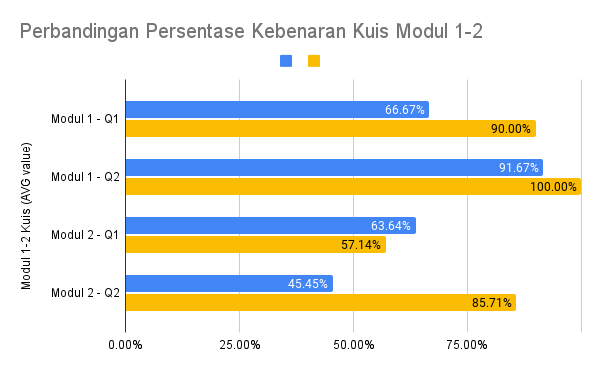
\includegraphics[width=0.85\textwidth]{chapter4/eksperimen-k1k2-kebenaran-all.png}
  \caption{Hasil eksperimen modul 1-2 soal kuis} \label{fig:eksperimen-k1k2-kebenaran-all}
  Sumber: Penulis (2022)
\end{figure}
\begin{figure}[H]
  \centering
  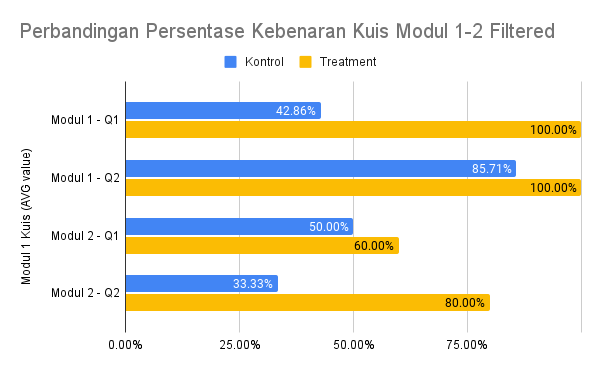
\includegraphics[width=0.85\textwidth]{chapter4/eksperimen-k1k2-kebenaran-awam.png}
  \caption{Hasil eksperimen modul 1-2 soal kuis setelah penyaringan data} \label{fig:eksperimen-k1k2-kebenaran-awam}
  Sumber: Penulis (2022)
\end{figure}

Berdasarkan pada \autoref{fig:eksperimen-k1k2-kebenaran-all} dan \autoref{fig:eksperimen-k1k2-kebenaran-awam} di atas, dapat dilihat bahwa hasil persentase kuis dengan jawaban yang benar pada grup perlakuan (\textit{treatment}) lebih tinggi rata-ratanya dibandingkan grup kontrol. Terdapat pengecualian pada modul 2 kuis 1 data keseluruhan karena terdapat data \textit{outlier}, tetapi setelah data disaring hasil persentase menjadi lebih konsisten.

Selain dari hasil persentase jawaban, dapat dilihat juga pada \autoref{fig:eksperimen-k1k2-waktu} yang dirangkum dari \autoref{appendix:data-modul1-waktu} dan \autoref{appendix:data-modul2-waktu} bahwa waktu pengerjaan kuis grup perlakuan jauh lebih lama dibanding waktu pengerjaan kuis grup kontrol karena peserta melakukan eksplorasi terlebih dahulu pada ILE yang disediakan.

\begin{figure}[H]
  \centering
  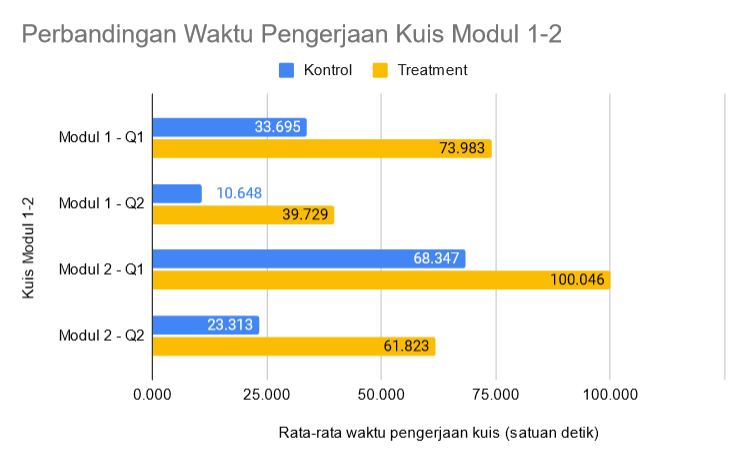
\includegraphics[width=0.85\textwidth]{chapter4/eksperimen-k1k2-waktu.png}
  \caption{Waktu menjawab soal kuis modul 1-2} \label{fig:eksperimen-k1k2-waktu}
  Sumber: Penulis (2022)
\end{figure}

\subsubsection{Analisis Data Eksperimen Soal Latihan Kode}

Dari data eksperimen soal latihan kode pada \autoref{appendix:data-modul1-jawaban} dan \autoref{appendix:data-modul2-jawaban}, didapatkan data-data eksperimen soal kuis modul 1 dan 2 sebagai \autoref{fig:eksperimen-lk1-all} dan \autoref{fig:eksperimen-lk1-awam} berikut.

\begin{figure}[H]
  \centering
  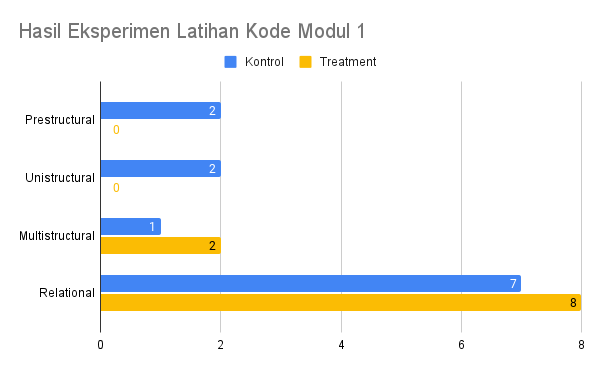
\includegraphics[width=0.85\textwidth]{chapter4/eksperimen-lk1-all.png}
  \caption{Hasil eksperimen modul 1 soal latihan kode} \label{fig:eksperimen-lk1-all}
  Sumber: Penulis (2022)
\end{figure}
\begin{figure}[H]
  \centering
  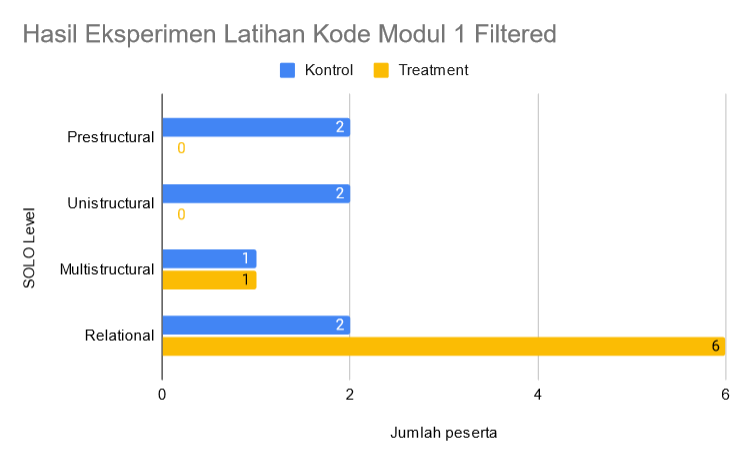
\includegraphics[width=0.85\textwidth]{chapter4/eksperimen-lk1-awam.png}
  \caption{Hasil eksperimen modul 1 soal latihan kode setelah penyaringan data} \label{fig:eksperimen-lk1-awam}
  Sumber: Penulis (2022)
\end{figure}

Berdasarkan pada \autoref{fig:eksperimen-lk1-all}, dapat dilihat bahwa pada grup perlakuan terdapat lebih banyak peserta yang mendapatkan nilai SOLO Level yang lebih tinggi dengan rata-rata SOLO Level grup perlakuan adalah 3.8 dan rata-rata SOLO Level grup kontrol adalah 3.083. Namun, apabila digunakan \textit{T test} independen dengan asumsi normal distribusi pada data, didapatkan nilai t sebesar 2.086 (\textit{p = 0.097}) yang berarti secara statistik dampak ILE terhadap hasil latihan kode modul 1 tidak terlalu signifikan. Maka dari itu, dilakukan penyaringan data untuk menghilangkan data \textit{outlier} yang dapat mempengaruhi hasil eksperimen. Dapat dilihat pada \autoref{fig:eksperimen-lk1-awam} data yang sudah disaring memiliki perubahan yang cukup besar dengan rata-rata SOLO Level grup perlakuan menjadi 3.857 dan rata-rata SOLO Level grup kontrol menjadi 2.429. Jika dilakukan \textit{T test} pada data yang sudah disaring, didapatkan nilai t sebesar 2.179 (\textit{p = 0.0147}) yang berarti secara statistik dampak ILE terhadap hasil latihan kode modul 1 signifikan.

Dari data eksperimen soal latihan kode pada \autoref{appendix:data-modul1-jawaban} dan \autoref{appendix:data-modul2-jawaban}, didapatkan data-data eksperimen soal kuis modul 1 dan 2 sebagai \autoref{fig:eksperimen-lk2-all} dan \autoref{fig:eksperimen-lk2-awam} berikut.

\begin{figure}[H]
  \centering
  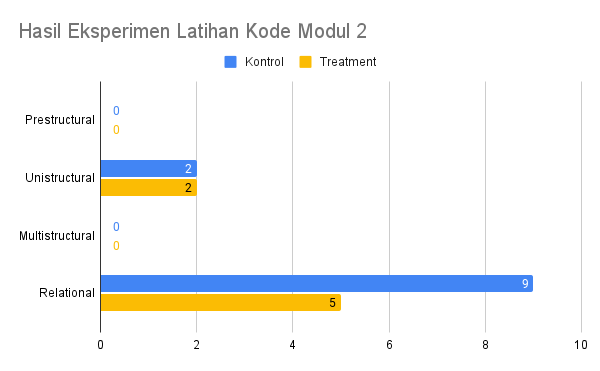
\includegraphics[width=0.85\textwidth]{chapter4/eksperimen-lk2-all.png}
  \caption{Hasil eksperimen modul 2 soal latihan kode} \label{fig:eksperimen-lk2-all}
  Sumber: Penulis (2022)
\end{figure}
\begin{figure}[H]
  \centering
  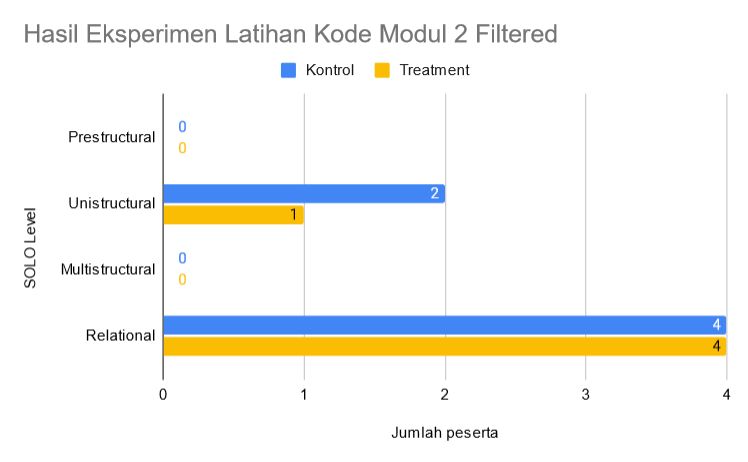
\includegraphics[width=0.85\textwidth]{chapter4/eksperimen-lk2-awam.png}
  \caption{Hasil eksperimen modul 2 soal latihan kode setelah penyaringan data} \label{fig:eksperimen-lk2-awam}
  Sumber: Penulis (2022)
\end{figure}

Berdasarkan pada \autoref{fig:eksperimen-lk2-all}, rata-rata SOLO Level grup perlakuan adalah 3.429 dan rata-rata SOLO Level grup kontrol adalah 3.636 sehingga grup kontrol memiliki hasil yang lebih tinggi dibanding grup perlakuan. Maka dari itu, dilakukan penyaringan data sehingga data berubah menjadi seperti pada \autoref{fig:eksperimen-lk1-awam}. Data yang sudah disaring memiliki perubahan yang cukup besar dengan rata-rata SOLO Level grup perlakuan menjadi 3.6 dan rata-rata SOLO Level grup kontrol menjadi 3.333 sehingga membuat grup perlakuan memiliki hasil rata-rata yang lebih tinggi dibanding grup kontrol. Namun, jika dilakukan \textit{T test} pada data yang sudah disaring, didapatkan nilai t sebesar 2.262 (\textit{p = 0.662}) yang berarti secara statistik dampak ILE terhadap hasil latihan kode modul 2 tidak signifikan. Salah satu faktor yang menyebabkan hal ini terjadi adalah kurangnya data akibat adanya peserta yang tidak menyelesaikan modul 2 eksperimen. Faktor lain yang dapat berpengaruh pada hasil ini adalah soal yang dibuat kurang bagus sehingga mempengaruhi hasil akhir dari eksperimen.

\subsubsection{Analisis Data Eksperimen Waktu Pengerjaan}
Seperti yang sempat dibahas sebelumnya pada \autoref{fig:eksperimen-k1k2-waktu}, terdapat pola bahwa waktu pengerjaan grup perlakuan jauh lebih lama dibanding grup kontrol. Hal ini dapat dilihat lebih lengkap pada \autoref{fig:eksperimen-m1m2-waktu} yang menampilkan perbandingan rata-rata waktu pengerjaan pada materi, soal kuis, dan soal latihan kode pada modul 1 dan modul 2. Lamanya pengerjaan modul pada grup perlakuan juga menjadi faktor yang membuat grup perlakuan lebih banyak yang tidak menyelesaikan modul 2 dan 3. Setelah diinvestigasi lebih lanjut, ditemukan pada beberapa peserta bahwa ILE dapat menjadi distraksi dalam pembelajaran karena peserta terlalu lama melakukan eksplorasi pada ILE sehingga tidak dapat menyelesaikan modul tepat waktu. Hasil olahan data diperoleh dari \autoref{appendix:data-modul1-waktu} dan \autoref{appendix:data-modul2-waktu}.

\begin{figure}[H]
  \centering
  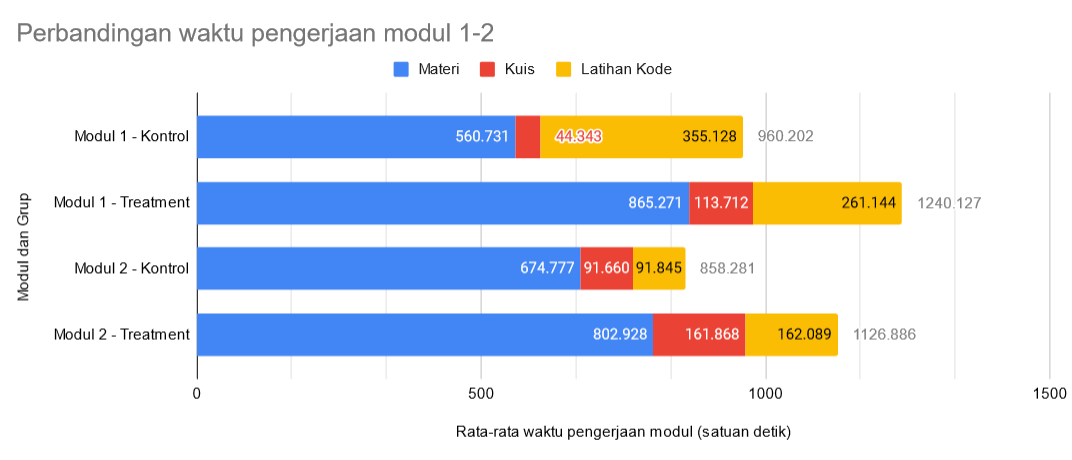
\includegraphics[width=0.85\textwidth]{chapter4/eksperimen-m1m2-waktu.png}
  \caption{Perbandingan waktu pengerjaan modul 1 dan modul 2} \label{fig:eksperimen-m1m2-waktu}
  Sumber: Penulis (2022)
\end{figure}

\subsection{Ancaman Validitas (Threat of Validity)}

Pada Laporan Tugas Akhir ini, terdapat beberapa ancaman validitas yang dapat mempengaruhi hasil dari pengujian:
\begin{enumerate}
  \item Pembelajaran hanya dilakukan selama 1 jam sehingga peserta tidak dapat menyelesaikan modul pembelajaran.
  \item Pembelajaran hanya membahas materi dasar agar dapat dipahami dan diselesaikan oleh orang awam. Hal ini membuat pemahaman awal pelajar menjadi krusial karena apabila pelajar telah mempelajari pemrograman sebelumnya, akan timbul data \textit{outlier} yang dapat mempengaruhi hasil eksperimen.
  \item Sulitnya mendapatkan peserta eksperimen dengan pemahaman konsep awal yang sama rata.
  \item Pembuatan materi pembelajaran tidak menggunakan tenaga kerja ahli.
  \item Jumlah sampel yang sedikit dan tidak memenuhi keseluruhan demografis pengguna KodeBareng karena menggunakan teknik \textit{convenience sampling}.
  \item Penilaian jawaban berdasarkan SOLO Level tidak menggunakan tenaga kerja ahli independen.
\end{enumerate}